\chapter{Density, plain, sparse and strict}\label{ch:density}

You said you did not understand this part. It is the most confusing part of the project, so we go
slowly. These are the four words to learn:

\begin{center}
\begin{tabularx}{\textwidth}{lX}
\toprule
Word & Meaning \\
\midrule
\textbf{Density} & The fraction of code values that are not exactly zero \\
\textbf{Plain} & Thresholds may fall as low as zero. Nothing stops them. Loss is MSE \\
\textbf{Sparse} & Thresholds are forbidden to fall below their starting value. Our addition \\
\textbf{Strict} & The same as plain, run at 32 and 64 layers, with nothing added \\
\bottomrule
\end{tabularx}
\end{center}

\section{What density is}

The network's final codes $x$ form a huge array: 32 maps of $768\times768$ values. Sparse coding promises
that almost all of them are zero. Density measures how true that is.

\begin{code*}{train_csc_lista.py}
                density = float((model.codes(sample) != 0).float().mean())
\end{code*}

So a density of 2\% means 98\% of the values are exactly zero. A density of 100\% means none are.
Our classical reference is the dictionary's own 2.4\%, from Chapter~\ref{ch:dictionary}.

\section{What went wrong}

The first full run had no restrictions: Eq.~20, MSE, 16 layers. It worked well, scoring 39.1\% on COMSOL. But
look at its density.

\begin{center}
\begin{tabular}{ll}
\toprule
Training step & Density \\
\midrule
0 (before training) & 20\% \\
250 & 99.9\% \\
\bottomrule
\end{tabular}
\end{center}

Within 250 steps, the code went from fairly sparse to completely full. The likely reason is simple.
Nothing in the MSE loss rewards sparsity. It only asks for a good output. Shrinking throws information
away, so training finds that the output improves when $\theta$ gets smaller. In the strict 32-layer
model, 6 of 32 thresholds hit exactly zero, and 19 others fell below the start. Only 7 rose.

\begin{figure}[H]
\centering
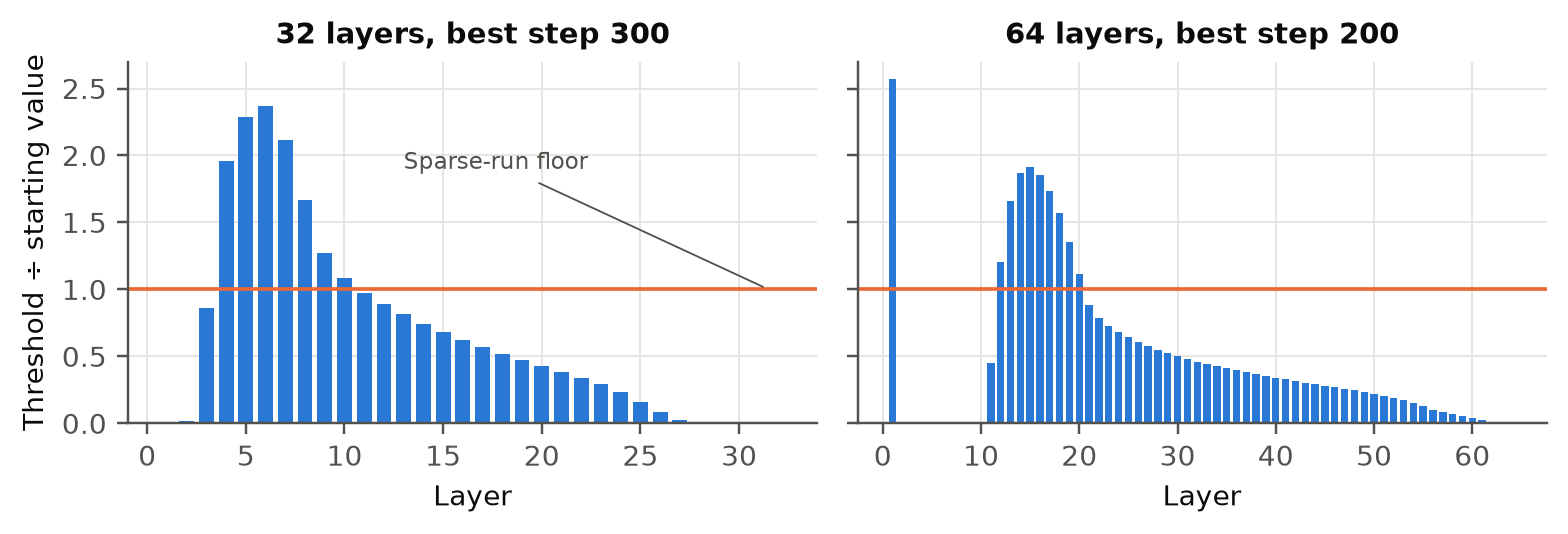
\includegraphics[width=\textwidth]{thresholds}
\caption{Learned threshold in each layer, divided by its starting value $\lambda/L$, for the two strict
models at their best step. The orange line at 1 is the lowest value allowed in sparse runs. No visible
bar means zero or nearly zero: the logs count 6 of 32 and 9 of 64 thresholds as exactly zero.}
\label{fig:thresholds}
\end{figure}

\begin{keyidea}[What a zero threshold means]
The logs print ``zero thresholds 6/32''. That counts layers with $\theta\le0$. With $\theta=0$, the shrink
function does nothing at all: $\soft_0(x)=x$. That layer is purely linear.
\end{keyidea}

\begin{careful}[The density number mostly reflects the last layer]
Density is measured on the final $x$, and the last step of the network is a shrink with $\theta^{(K)}$. If
that one threshold is zero, then almost no value is exactly zero, however the earlier layers behaved. In the
strict 32-layer model the last threshold is exactly 0, and density is about 100\%. In the strict 64-layer
model it is tiny but not zero, and density jumps around between 73\% and 99\% from checkpoint to checkpoint.
So treat this number as a coarse signal, not a precise measure.
\end{careful}

\section{So what is the network actually doing?}

At density near 100\%, with some thresholds at zero, there is little sparse coding left. The network acts
mostly as a \textbf{learned, nearly linear deconvolution}: a deep stack of filters. It starts as ISTA, and it uses
the ISTA structure as a good starting shape. But the final object is not finding a few active atoms.

\begin{defend}
\textbf{``Is this still sparse coding?''} Be honest: the structure is, the behaviour mostly is not. Do not
describe the strict models as sparse. The accurate sentence is: ``It is Eq.~20 of Liu et al., but
after MSE training the codes are dense, so it behaves like a learned deconvolution.''
\end{defend}

\section{Sparse runs: an attempt to fix it}

To force sparsity, I added one option that keeps thresholds at or above a floor.

\begin{code*}{train_csc_lista.py}
    floor = args.theta_floor * float(model.theta.min())
\end{code*}
\begin{code*}{train_csc_lista.py}
        with torch.no_grad():
            model.theta.clamp_(min=floor)
\end{code*}

This single flag is the difference between the names:

\begin{itemize}
\item \code{--theta-floor 0}: thresholds can reach zero. This is \textbf{plain}.
\item \code{--theta-floor 1}: thresholds stay at or above $\lambda/L$. This is \textbf{sparse}.
\end{itemize}

\textbf{There is no separate ``sparse Eq.~20'' in the paper.} Both are the same equation. Sparse is Eq.~20 plus my
constraint on one parameter. The result:

\begin{center}
\begin{tabular}{lcccc}
\toprule
16 layers, MSE & Density at best step & Simulated validation & COMSOL \\
\midrule
Plain & 99.9\% & 53.4\% & 39.1\% \\
Sparse & 28.8\% & 48.6\% & 40.2\% \\
\bottomrule
\end{tabular}
\end{center}

The floor worked in one sense: density fell to about 29\%, still far above the dictionary's 2.4\%. And it
helped on simulation. But it made COMSOL slightly \emph{worse}.

\section{Relative loss: a second attempt}

The MSE curves peaked at step 250 and then got worse, even though training continued. That pointed to a
mismatch between the loss and the metric. So the next runs used the relative loss, and added more layers.

\section{Every CSC-LISTA run in one table}

\begin{center}
\small
\begin{tabular}{lrrlcrrrr}
\toprule
Name & Layers & Steps & Loss & Floor & Best step & Density & Simulated & COMSOL \\
\midrule
Plain & 16 & 2,000 & MSE & no & 250 & 99.9\% & 53.4\% & 39.1\% \\
Sparse MSE & 16 & 2,000 & MSE & yes & 250 & 28.8\% & 48.6\% & 40.2\% \\
Sparse relative & 16 & 1,000 & Relative & yes & 1,000 & 25.6\% & 45.6\% & 42.0\% \\
Sparse relative & 32 & 1,000 & Relative & yes & 700 & 22.1\% & 42.5\% & 38.9\% \\
\textbf{Strict} & \textbf{32} & \textbf{1,000} & \textbf{MSE} & \textbf{no} & \textbf{300} & \textbf{99.9\%} & \textbf{51.9\%} & \textbf{35.4\%} \\
\textbf{Strict} & \textbf{64} & \textbf{1,000} & \textbf{MSE} & \textbf{no} & \textbf{200} & \textbf{74.2\%} & \textbf{48.8\%} & \textbf{33.8\%} \\
\bottomrule
\end{tabular}
\end{center}

Density is the value logged at the best step. Plain and strict have the same settings, apart from the number of
layers, the length of the run, and how often validation ran: every 250 steps for plain and every 100 for strict. The
Eq.~20 layer is identical in both code versions.

\begin{figure}[H]
\centering
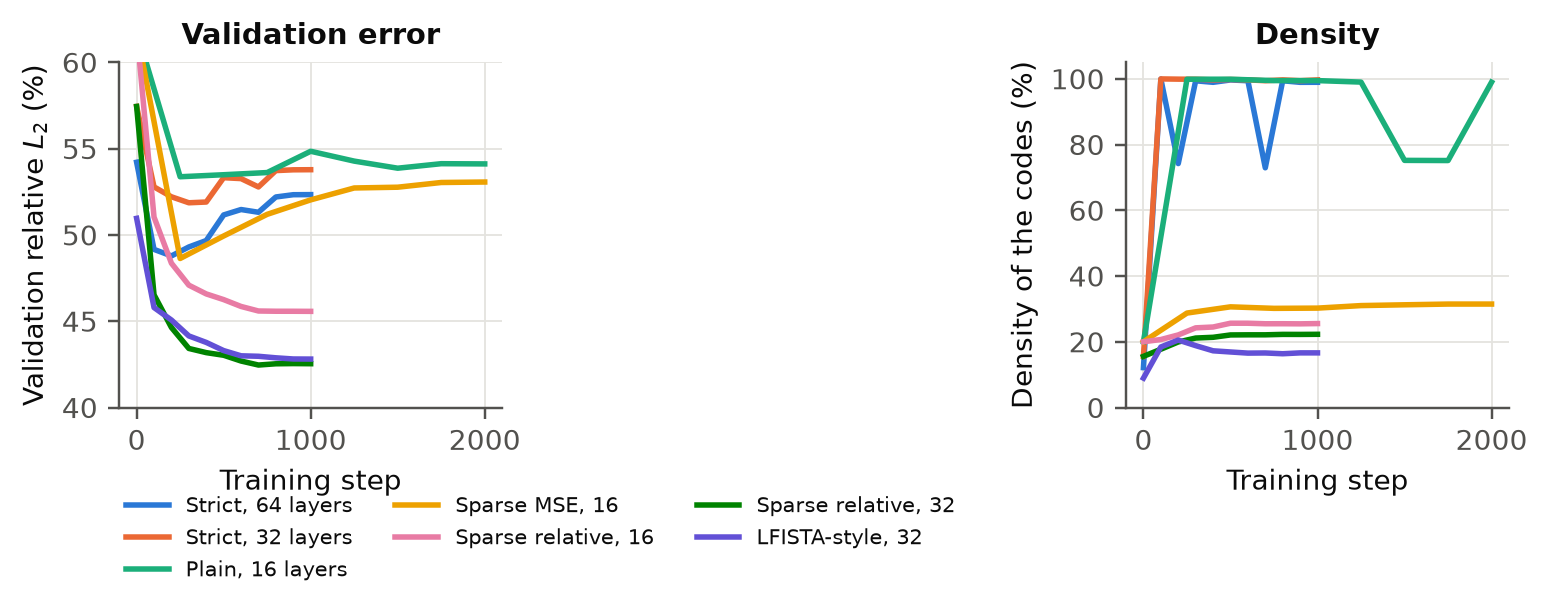
\includegraphics[width=\textwidth]{curves}
\caption{Validation error and density during training. Plain and strict runs jump to near 100\% density almost
at once. Sparse runs stay low. MSE runs reach their best validation error early, then get worse.}
\label{fig:curves}
\end{figure}

\section{Why ``strict'' exists}

After the sparse runs you asked whether everything was exactly what the paper did, because you cannot
defend additions. The honest answer was no. So we removed the floor and the relative loss, and reran
Eq.~20 as closely as we could at 32 and 64 layers. You also asked why rerun 32 layers when it had already
run. The earlier 32-layer run had the floor and the relative loss, so it was not strict.

And here is the surprise.

\begin{keyidea}[The result you should remember]
Removing my additions made the COMSOL score better: 38.9\% became 35.4\% at the same 32 layers. The sparse
version looked far better on simulated validation, but lost on COMSOL. Simpler was better, and it is
also more defensible.
\end{keyidea}

\section{What the later runs add to this story}

Two later results change how to think about density.

\textbf{Dense codes are not required.} The LFISTA-style network of Chapter~\ref{ch:lfista} is trained on the Lasso objective,
which includes the $\ell_1$ penalty, so its loss does reward sparsity. Its density stayed at 16.6\%, none of its 32
thresholds reached zero, and it still scored 34.2\%, close to strict 64 layers. This suggests the loss decides it: MSE lets
the codes fill up, and Lasso keeps them sparse. That is one run of each, so treat it as a strong hint.

\textbf{Our best method is not very sparse either.} On the crop in Figure~\ref{fig:reconstruction}, FISTA-300 with
$\lambda=0.009$ has a density of 27.6\%. The dictionary's 2.4\% came from fitting sharp fields with $\lambda=0.3$, which is a
different problem. So 2.4\% is not a fair target for deblurring.
